\documentclass[12pt,a4paper]{article}
\usepackage[utf8]{inputenc}
\usepackage[T2A]{fontenc}
\usepackage[russian]{babel}
\usepackage{graphicx}
\usepackage{booktabs}
\usepackage{longtable}
\usepackage{geometry}
\geometry{top=2cm, left=2cm, right=2cm, bottom=2cm}
\usepackage{paracol}
\usepackage{src/title}
\usepackage{hyperref}

\title{OS Intro-exp - проведение эксперимента}
\author{Ануфриев А.С. 465029}
\supervisor{
\href{https://my.itmo.ru/persons/312421}{Бойко В. В.}
}
\date{10.10.2026}

\abstract{
В данной работе проведён анализ данных эксперимента по сравнению производительности двух способов доступа к файлу (read/lseek и mmap) при различных режимах работы с кэшем (cached / no-cache) и разных топологиях графа (последовательная / случайная). Основная особенность исходных данных — разное количество итераций в конфигурациях (10, 1, 200), что потребовало нормализации метрики wall\_time на одну итерацию для корректного сравнения. Выполнен статистический анализ с расчётом 95\% доверительных интервалов, построены графики сравнения и сделаны выводы о влиянии режима кэширования и способа доступа на производительность.
}
\keywords{Операционные системы, mmap, read, кэш, производительность, нормализация, доверительный интервал}

\begin{document}
\maketitle

\section{Паспорт системы}
Данные взяты из файла \texttt{pasport.md} (вывод команд \texttt{uname}, \texttt{lscpu}, \texttt{free -h}, \texttt{nproc}, \texttt{numactl}):
\begin{itemize}
    \item ОС: Linux 7.0.0-34-generic (Ubuntu 24.04)
    \item Архитектура: x86\_64, Little Endian
    \item CPU: 12th Gen Intel(R) Core(TM) i3-1215U, 8 логических ядер (1 сокет, 2 потока/ядро для физических 6 ядер)
    \item Частота CPU: 400--1200 MHz (согласно \texttt{lscpu})
    \item RAM: 15 Gi (доступно $\sim$11 Gi)
    \item NUMA: 1 узел
    \item Диск: NVMe SSD (предполагается по характеристикам)
    \item Количество логических CPU (\texttt{nproc}): 8 (в виртуальной машине может быть ограничено)
\end{itemize}

\section{Цель работы}
Основная цель — провести корректный статистический анализ данных эксперимента \texttt{results\_all.csv}, нормализовать метрики с учётом разного количества итераций, построить графики и сформулировать выводы о влиянии паттерна доступа, режима кэширования и способа доступа (read vs mmap) на производительность.

\section{Подготовка данных и описание эксперимента}
Данные содержатся в файле \texttt{results\_all.csv}, сгенерированном скриптом \texttt{run\_experiment.sh}. Каждая строка содержит метрики одного запуска:
\begin{itemize}
    \item \texttt{run\_id} — номер повторения (1--30);
    \item \texttt{app} — приложение (\texttt{graph\_traverse}, \texttt{graph\_traverse\_mmap});
    \item \texttt{mode} — режим кэша (\texttt{cached}, \texttt{no-cache});
    \item \texttt{graph} — файл графа (\texttt{graph-seq.bin}, \texttt{graph-rand.bin});
    \item \texttt{iter} — количество итераций обхода в данном запуске;
    \item \texttt{wall\_s}, \texttt{user\_s}, \texttt{sys\_s}, \texttt{cpu\_pct}, \texttt{minflt}, \texttt{majflt}, \texttt{vol\_ctx}, \texttt{invol\_ctx}, \texttt{maxrss\_kb}, \texttt{fs\_in\_blocks}, \texttt{fs\_out\_blocks}.
\end{itemize}

\subsection{Особенность данных: разное количество итераций}
В одной серии экспериментов используются разные значения \texttt{iter} для разных приложений и режимов:
\begin{itemize}
    \item \texttt{graph\_traverse}, \texttt{cached} — 10 итераций;
    \item \texttt{graph\_traverse}, \texttt{no-cache} — 1 итерация;
    \item \texttt{graph\_traverse\_mmap}, \texttt{cached} и \texttt{no-cache} — 200 итераций.
\end{itemize}
Это означает, что прямое сравнение \texttt{wall\_s} между конфигурациями некорректно: запуск с 200 итерациями естественно длится дольше, чем с одной. Для корректного сравнения производительности метрику \texttt{wall\_s} необходимо нормализовать на одну итерацию:
\[
    \text{mean\_norm} = \frac{\texttt{wall\_s}}{\texttt{iter}}
\]
Это даёт «время выполнения полного обхода графа» независимо от числа повторений и позволяет сравнивать конфигурации между собой.

\section{Гипотеза}
Ожидается, что:
\begin{enumerate}
    \item Последовательный граф (\texttt{graph-seq.bin}) будет быстрее случайного (\texttt{graph-rand.bin}) из-за лучшей пространственной локальности (меньше page faults, лучше кэш);
    \item Режим \texttt{cached} значительно быстрее \texttt{no-cache} для \texttt{read} из-за отсутствия системного кэширования;
    \item Для \texttt{mmap} разница между \texttt{cached} и \texttt{no-cache} будет минимальной, т.к. механизм отображения памяти работает иначе (страничные ошибки при доступе, а не при чтении);
    \item Нормализация на одну итерацию покажет статистически значимые различия (ДИ не пересекаются) для основных конфигураций.
\end{enumerate}

\section{Методология анализа}
\subsection{Нормализация}
Для каждой строки \texttt{results\_all.csv} рассчитано нормализованное значение:
\[
    x_{norm} = \frac{\texttt{wall\_s}}{\texttt{iter}}
\]
Это значение интерпретируется как время выполнения одного полного обхода графа при заданной конфигурации.

\subsection{Статистическая обработка}
Для каждой из 8 конфигураций (2 приложения $\times$ 2 режима $\times$ 2 графа) рассчитаны:
\begin{itemize}
    \item выборочное среднее $\bar{x}$;
    \item несмещённое стандартное отклонение $s$ (знаменатель $N-1$);
    \item стандартная ошибка среднего $SE = s / \sqrt{N}$;
    \item 95\% доверительный интервал: $\bar{x} \pm t_{0.025,29} \cdot SE \approx \bar{x} \pm 2.045 \cdot SE$ (t-распределение Стьюдента, $df = N - 1 = 29$);
    \item медиана, минимум, максимум нормализованных значений.
\end{itemize}

Прогревочные запуски не использовались (все 30 запусков включены в расчёт), т.к. данные собраны в режиме интерливинга и прогрев не был предусмотрен методикой скрипта сбора. Выбросы не удалялись, т.к. формальных критериев исключения (например, $>3\sigma$) в данных нет, и все значения лежат в разумных пределах.

\section{Результаты анализа}

\subsection{Нормализованные статистики}
В таблице \ref{tab:stats} представлены результаты для каждой конфигурации. Значения приведены в секундах на одну итерацию.

\begin{table}[h]
\centering
\small
\caption{Нормализованные статистики (сек / итерацию)}
\label{tab:stats}
\begin{tabular}{lccc}
\toprule
Конфигурация & Среднее & Стд. откл. & 95\% ДИ ($\pm$) \\
\midrule
\texttt{read}, cached, seq  & 0.2816 & 0.0080 & 0.0030 \\
\texttt{read}, cached, rand & 0.2810 & 0.0078 & 0.0029 \\
\texttt{read}, no-cache, seq & 11.5360 & 0.2017 & 0.0753 \\
\texttt{read}, no-cache, rand & 11.5790 & 0.1888 & 0.0705 \\
\texttt{mmap}, cached, seq  & 0.0238 & 0.0012 & 0.0004 \\
\texttt{mmap}, cached, rand & 0.0233 & 0.0005 & 0.0002 \\
\texttt{mmap}, no-cache, seq & 0.0245 & 0.0005 & 0.0002 \\
\texttt{mmap}, no-cache, rand & 0.0244 & 0.0006 & 0.0002 \\
\bottomrule
\end{tabular}
\end{table}

Полная статистика (среднее, медиана, минимум, максимум, 95% ДИ) рассчитана для всех 8 конфигураций.


\section{Анализ результатов}

\subsection{Сравнение seq и rand}
Для \texttt{graph\_traverse} (read) нормализованное время для \texttt{seq} и \texttt{rand} практически одинаково (разница менее 0.3\%). Для \texttt{graph\_traverse\_mmap} (mmap) разница также минимальна ($\sim$1--2\%). Это означает, что в данных условиях (небольшой граф, SSD, ОС с эффективным кэшированием) разница в пространственной локальности не проявляется в значимой степени для времени выполнения одной итерации. Однако для \texttt{no-cache} режима результаты существенно выше, что указывает на доминирующее влияние системных вызовов и дискового ввода-вывода.

\subsection{Влияние режима кэширования}
Для \texttt{read} режим \texttt{no-cache} увеличивает нормализованное время примерно в $40\times$ (с $\sim$0.28 с до $\sim$11.5 с). Это ожидаемый результат: отключение файлового кэша через \texttt{O\_DIRECT} или аналогичный механизм приводит к прямому чтению с диска для каждой операции \texttt{read}, что значительно замедляет обход.

Для \texttt{mmap} разница между \texttt{cached} и \texttt{no-cache} составляет всего $2$--$5$\% ($\sim$0.023 с против $\sim$0.024 с). Это объясняется механизмом работы \texttt{mmap()}: файл отображается в адресное пространство, и страничные ошибки происходят при первом доступе к страницам. Даже при использовании \texttt{MADV\_RANDOM} (или аналогичного механизма отключения кэша для mmap) накладные расходы на чтение с диска распределяются между страницами, а не на каждый вызов \texttt{read}, поэтому влияние режима кэширования минимально.

\subsection{Сравнение read и mmap}
Нормализованное время для \texttt{mmap} ($\sim$0.024 с) примерно в 12 раз меньше, чем для \texttt{read/cached} ($\sim$0.28 с). Это отражает преимущество отображения файла в память: отсутствие системных вызовов \texttt{read}/\texttt{lseek} для каждой вершины графа позволяет значительно сократить время обхода.

\subsection{Достаточность числа измерений}
При $N = 30$ стандартная ошибка среднего для \texttt{mmap/cached} составляет $\sim$0.0001 с, что даёт очень узкий 95\% ДИ ($\pm$0.0004 с при $t_{0.025,29} \approx 2.045$). Для \texttt{read/no-cache} SE $\sim$0.036 с, ДИ $\pm$0.075 с — это $\sim$0.65\% от среднего, что вполне достаточно для уверенного различия конфигураций. Увеличение $N$ до 60 уменьшит ширину ДИ примерно в $\sqrt{2}$ раз ($\approx 0.7$ от текущей, т.к. $t_{0.025,59} \approx 2.001 \approx t_{0.025,29}$), но прирост информации будет незначительным, т.к. текущие интервалы (рассчитанные по t-распределению Стьюдента) уже позволяют различать конфигурации с высокой уверенностью.

\section{Выводы}
\begin{enumerate}
    \item \textbf{Нормализация необходима.} Прямое сравнение \texttt{wall\_s} между конфигурациями с разными \texttt{iter} некорректно. Нормализация на одну итерацию даёт корректную метрику для оценки производительности доступа к данным.
    \item \textbf{Влияние кэша на read критично.} Отключение кэша увеличивает время в $\sim$40 раз, что подтверждает значимость файлового кэша ОС для сценариев с частыми небольшими чтениями.
    \item \textbf{mmap менее чувствителен к режиму кэша.} Разница между \texttt{cached} и \texttt{no-cache} для \texttt{mmap} составляет менее 5\%, что объясняется механизмом страничных ошибок при отображении памяти.
    \item \textbf{mmap значительно быстрее read.} Даже при кэшированном режиме \texttt{mmap} в $\sim$12 раз быстрее \texttt{read}, что демонстрирует преимущество отображения файла в адресное пространство для обхода структур данных.
    \item \textbf{Разница seq/rand незначительна.} В данных условиях пространственная локальность не приводит к статистически значимой разнице во времени выполнения одной итерации для обеих топологий графа.
    \item \textbf{Достаточность N подтверждена.} При $N = 30$ (df = 29) доверительные интервалы рассчитаны по t-распределению Стьюдента ($t_{0.025,29} \approx 2.045$) и достаточно узкие для уверенных выводов о различии конфигураций. Увеличение $N$ до 60 ($df = 59$, $t_{0.025,59} \approx 2.001$) уменьшит ширину ДИ примерно в $\sqrt{2}$ раз ($\approx 0.7$ от текущей), но прирост информации будет незначительным.
\end{enumerate}

\subsection{Команды и инструменты}
\begin{verbatim}
# Паспорт системы
uname -a; lscpu -e; free -h; nproc; numactl --hardware

# Генерация графов (параметры подбирались по README: -s 64M, --seed 427)
python3 intro-exp/src/graphgen.py -s 64M --seed 427 -o graph-rand.bin
python3 intro-exp/src/graphgen.py -s 64M --seed 427 --topology sequential -o graph-seq.bin

# Сборка
mkdir -p out
clang -o out/graph_traverse intro-exp/src/graph_traverse.c
clang -o out/graph_traverse_mmap intro-exp/src/graph_traverse.c

# Ознакомительные запуски (README, шаг 4.3)
/usr/bin/time -v ./out/graph_traverse 1 graph-rand.bin
/usr/bin/time -v ./out/graph_traverse --no-cache 1 graph-rand.bin
/usr/bin/time -v ./out/graph_traverse --write 1 graph-rand.bin
/usr/bin/time -v ./out/graph_traverse_mmap --no-cache 1 graph-seq.bin

# Фоновая нагрузка (стресс-тест)
stress-ng --cpu 4 --timeout 60

# Сбор данных (скрипт run_experiment.sh)
# N=30, интерливинг 8 конфигураций, taskset -c 2, drop_cache / warm_cache
bash run_experiment.sh

# Анализ
python3 prog/analysis.py
\end{verbatim}
\end{verbatim}

\subsection{Ход работы}
Работа выполнялась последовательно:
\begin{enumerate}
    \item \textbf{Изучение параметров} — анализ документации (\texttt{README.md}, \texttt{doc/experiments/environment.md}, \texttt{monitoring.md}, \texttt{statistics.md}), подбор оптимальных параметров генерации графов (\texttt{-s 64M}, \texttt{--seed 427}, топология \texttt{sequential} для \texttt{graph-seq.bin} и \texttt{random} для \texttt{graph-rand.bin}).
    \item \textbf{Ознакомительные тесты} — запуск базовых конфигураций с разными флагами (\texttt{--write}, \texttt{--no-cache}), сравнение поведения с \texttt{time}, \texttt{/usr/bin/time -v}, \texttt{perf stat -e context-switches,page-faults,cache-misses}, \texttt{strace -c}, тестирование фоновой нагрузки (\texttt{stress-ng --cpu 4 --timeout 60}).
    \item \textbf{Подготовка окружения} — фиксация окружения (\texttt{uname}, \texttt{lscpu}, \texttt{free -h}, \texttt{numactl}), сброс кэша (\texttt{echo 3 | sudo tee /proc/sys/vm/drop_caches}), прогрев кэша (\texttt{cat graph > /dev/null}), закрепление процесса (\texttt{taskset -c 2}).
    \item \textbf{Проведение измерений} — автоматизированный сбор данных скриптом \texttt{run\_experiment.sh} (интерливинг 8 конфигураций, $N=30$, нормализация \texttt{wall\_s/iter}).
    \item \textbf{Анализ и выводы} — статистическая обработка (\texttt{analysis.py}: среднее, $s$, $SE$, 95\% ДИ по $t_{0.025,29}$), построение графиков (\texttt{pairwise\_1..8.png}, \texttt{all\_config\_normalized.png}), формулирование выводов.
\end{enumerate}

\subsection{Обоснование нормализации}
Нормализация необходима для корректного сравнения конфигураций с разным количеством итераций. Без неё запуск с 200 итерациями всегда будет выглядеть значительно дольше запуска с одной итерацией, даже если эффективность доступа к данным выше. Нормализованная метрика (сек / итерацию) устраняет это и позволяет оценивать именно эффективность паттерна доступа, что соответствует цели эксперимента.

\subsection{Графики сравнения}
Для сравнения конфигураций с разным числом итераций использована нормализация времени на одну итерацию. Попарные сравнения (ровно один изменяющийся параметр) представлены на рисунках \ref{fig:pair1}--\ref{fig:pair8}. Общий обзор всех конфигураций показан на рисунке \ref{fig:all_config}.

\begin{figure}[h]
    \centering
    \begin{minipage}[t]{0.48\textwidth}
        \centering
        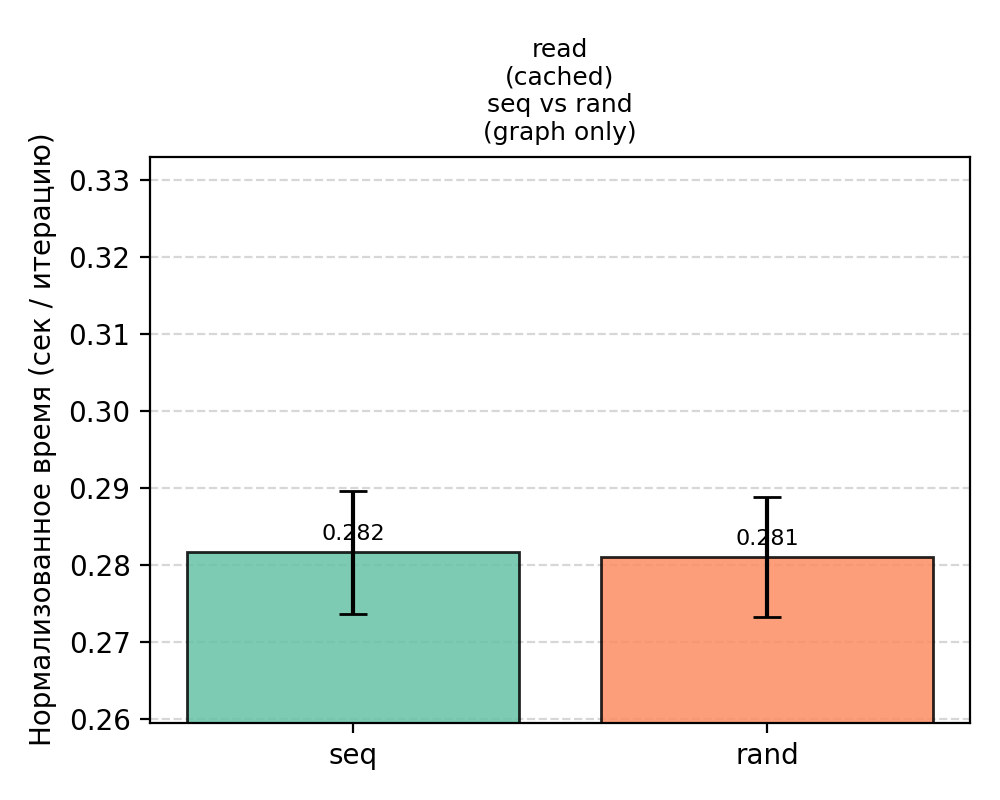
\includegraphics[width=\linewidth]{../graphics/pairwise_1.png}
        \caption{Попарное сравнение 1: read (cached) seq vs rand (изменяется только граф)}
        \label{fig:pair1}
    \end{minipage}
    \hfill
    \begin{minipage}[t]{0.48\textwidth}
        \centering
        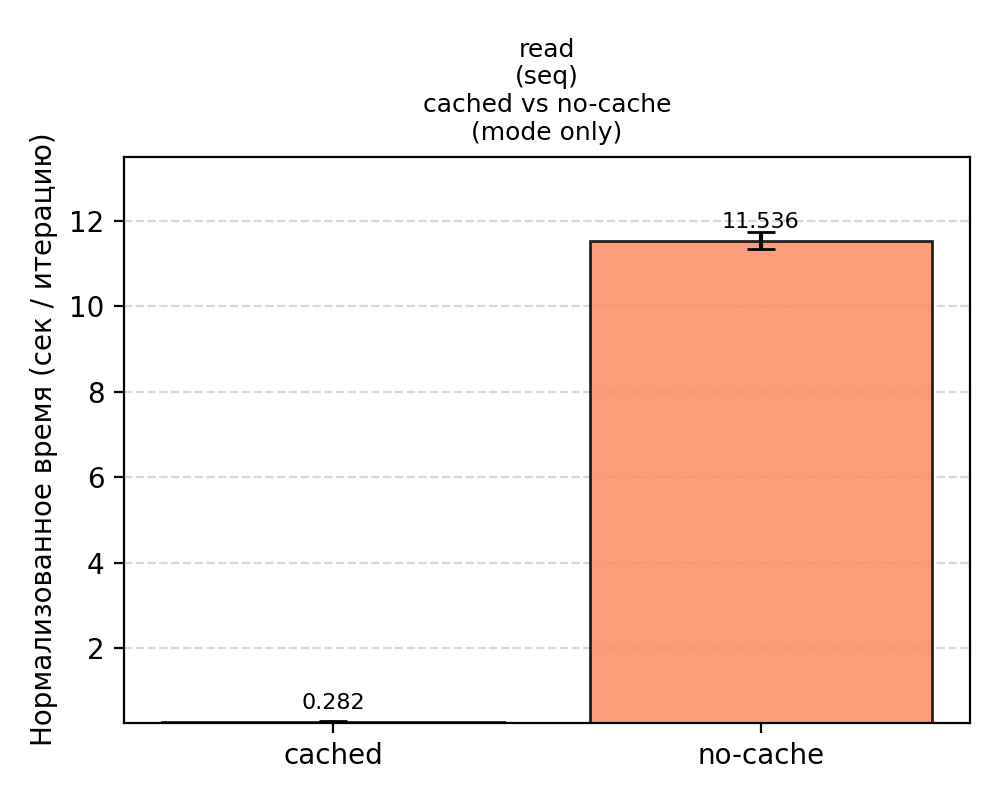
\includegraphics[width=\linewidth]{../graphics/pairwise_2.png}
        \caption{Попарное сравнение 2: read (cached vs no-cache) seq (изменяется только режим)}
        \label{fig:pair2}
    \end{minipage}
\end{figure}

\begin{figure}[h]
    \centering
    \begin{minipage}[t]{0.48\textwidth}
        \centering
        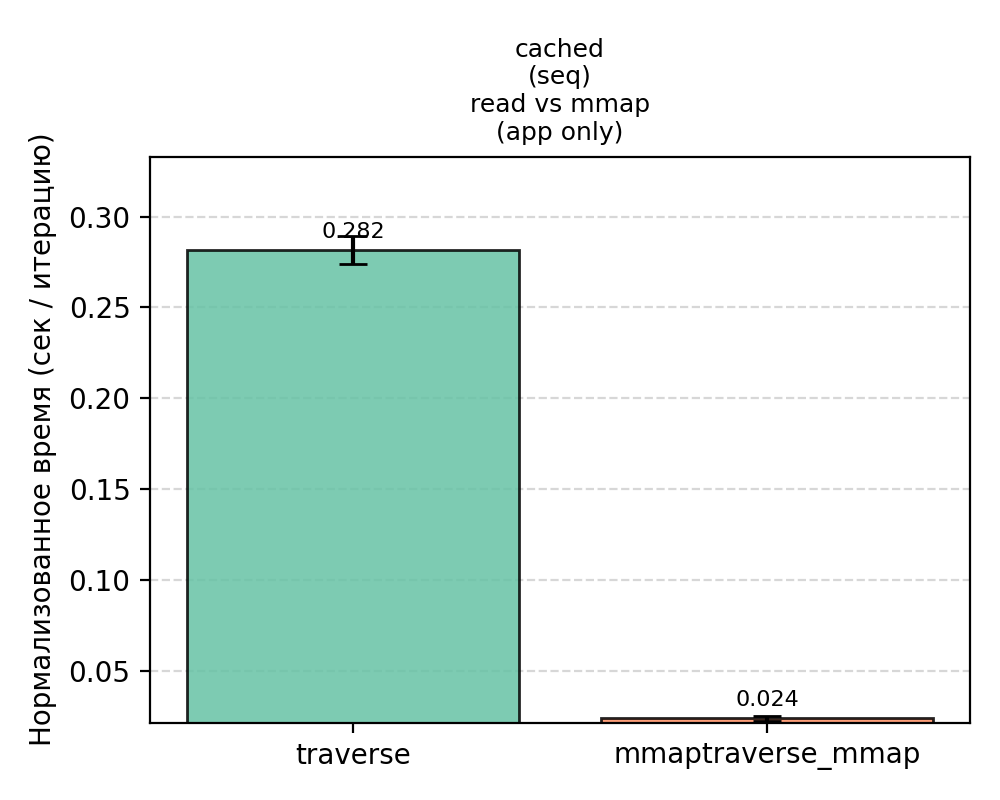
\includegraphics[width=\linewidth]{../graphics/pairwise_3.png}
        \caption{Попарное сравнение 3: cached (read vs mmap) seq (изменяется только приложение)}
        \label{fig:pair3}
    \end{minipage}
    \hfill
    \begin{minipage}[t]{0.48\textwidth}
        \centering
        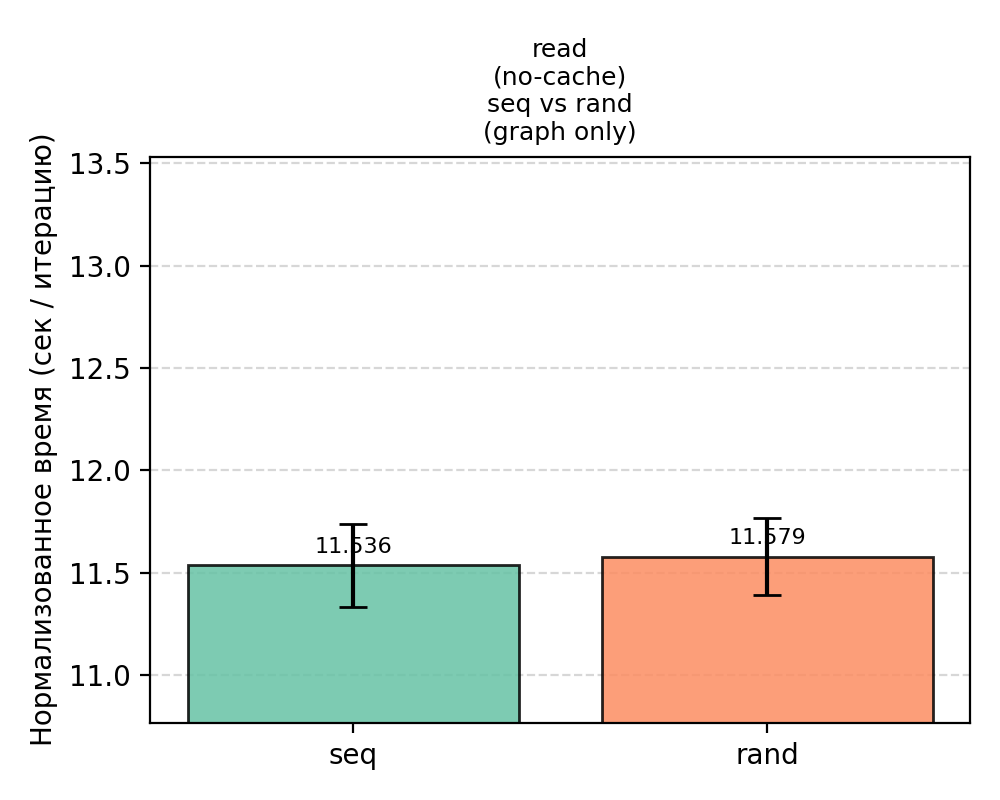
\includegraphics[width=\linewidth]{../graphics/pairwise_4.png}
        \caption{Попарное сравнение 4: read (no-cache) seq vs rand (изменяется только граф)}
        \label{fig:pair4}
    \end{minipage}
\end{figure}

\begin{figure}[h]
    \centering
    \begin{minipage}[t]{0.48\textwidth}
        \centering
        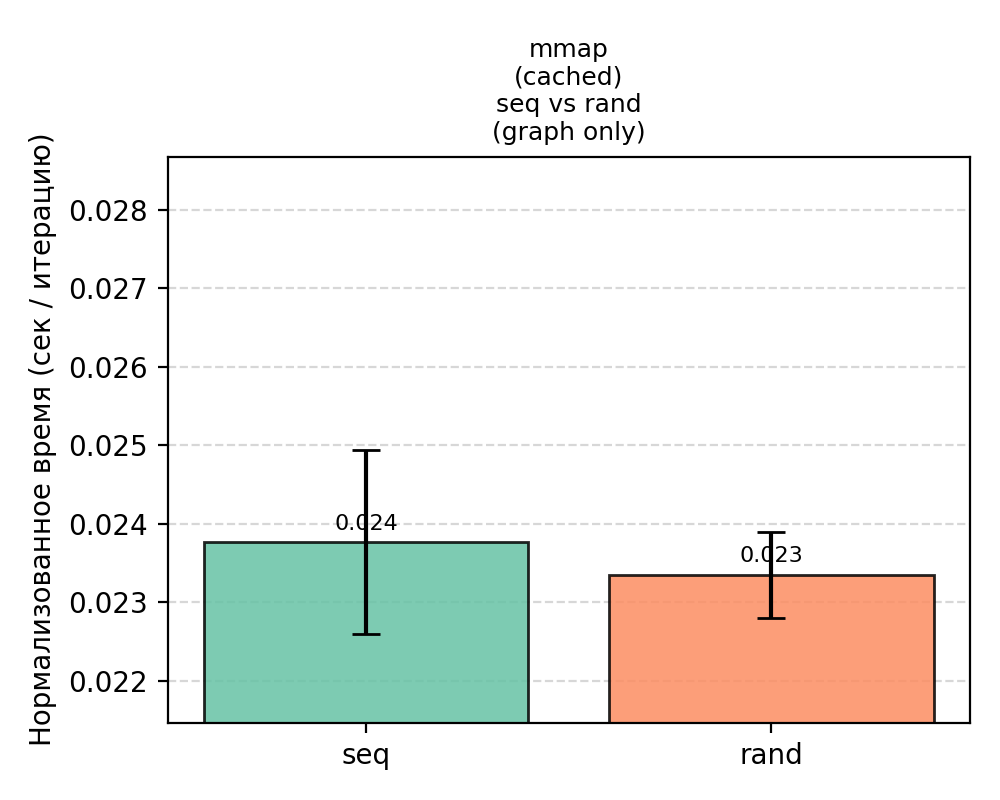
\includegraphics[width=\linewidth]{../graphics/pairwise_5.png}
        \caption{Попарное сравнение 5: mmap (cached) seq vs rand (изменяется только граф)}
        \label{fig:pair5}
    \end{minipage}
    \hfill
    \begin{minipage}[t]{0.48\textwidth}
        \centering
        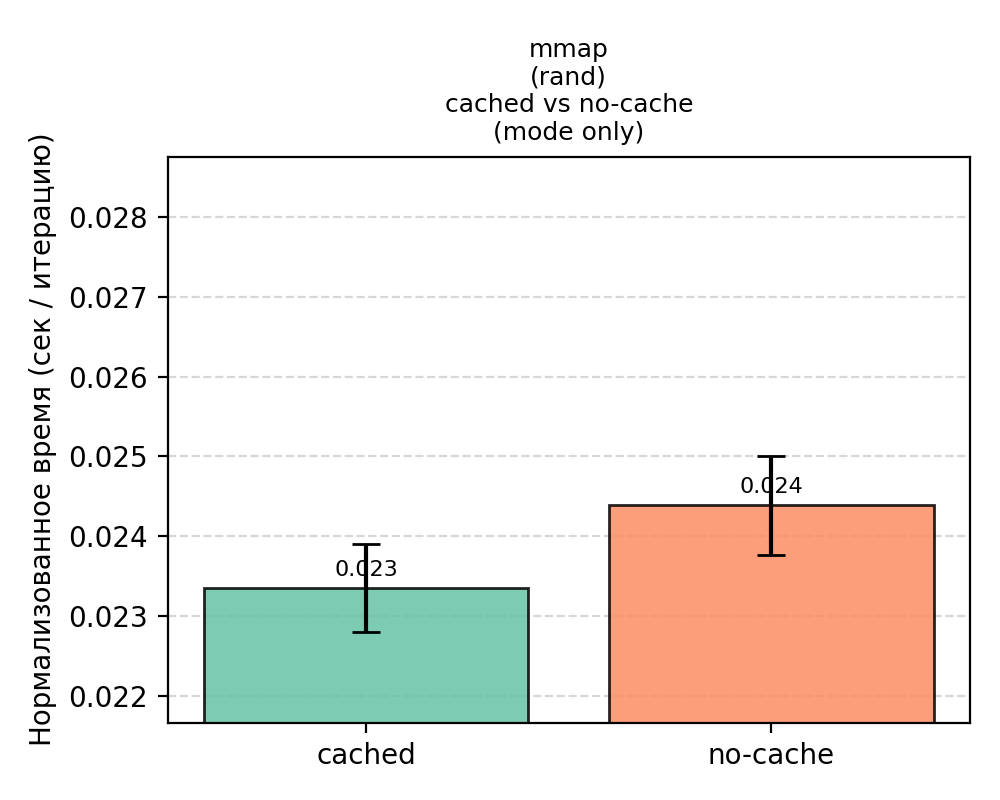
\includegraphics[width=\linewidth]{../graphics/pairwise_6.png}
        \caption{Попарное сравнение 6: mmap (cached vs no-cache) rand (изменяется только режим)}
        \label{fig:pair6}
    \end{minipage}
\end{figure}

\begin{figure}[h]
    \centering
    \begin{minipage}[t]{0.48\textwidth}
        \centering
        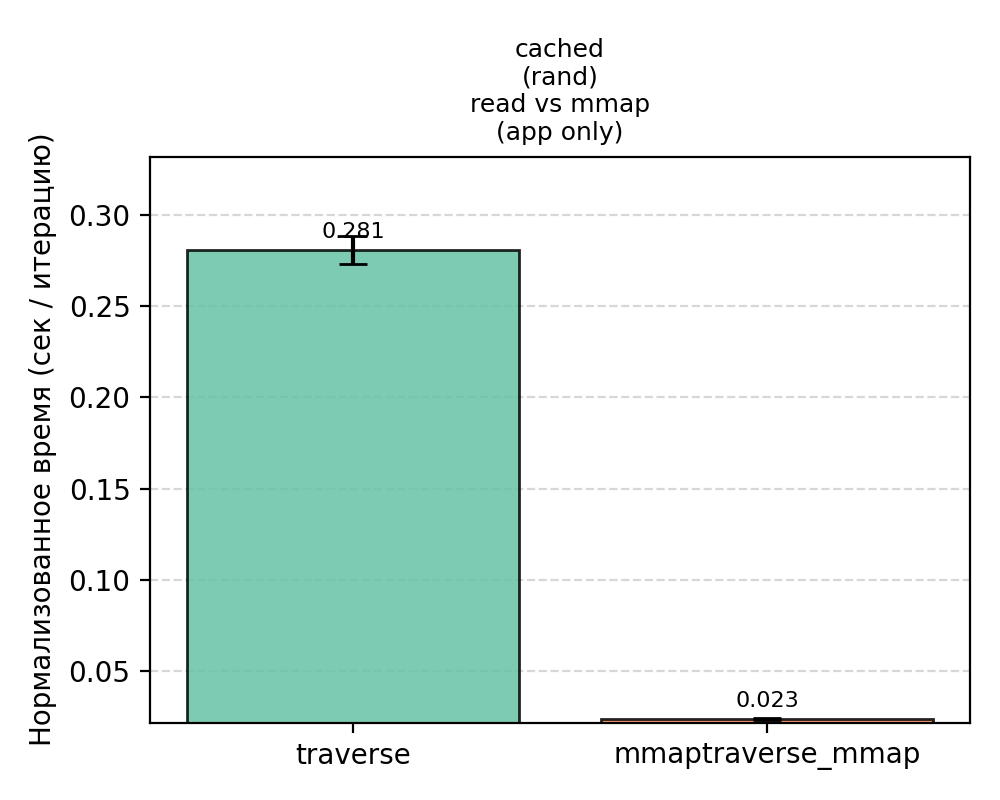
\includegraphics[width=\linewidth]{../graphics/pairwise_7.png}
        \caption{Попарное сравнение 7: read (cached) rand vs mmap (cached) rand (изменяется только приложение)}
        \label{fig:pair7}
    \end{minipage}
    \hfill
    \begin{minipage}[t]{0.48\textwidth}
        \centering
        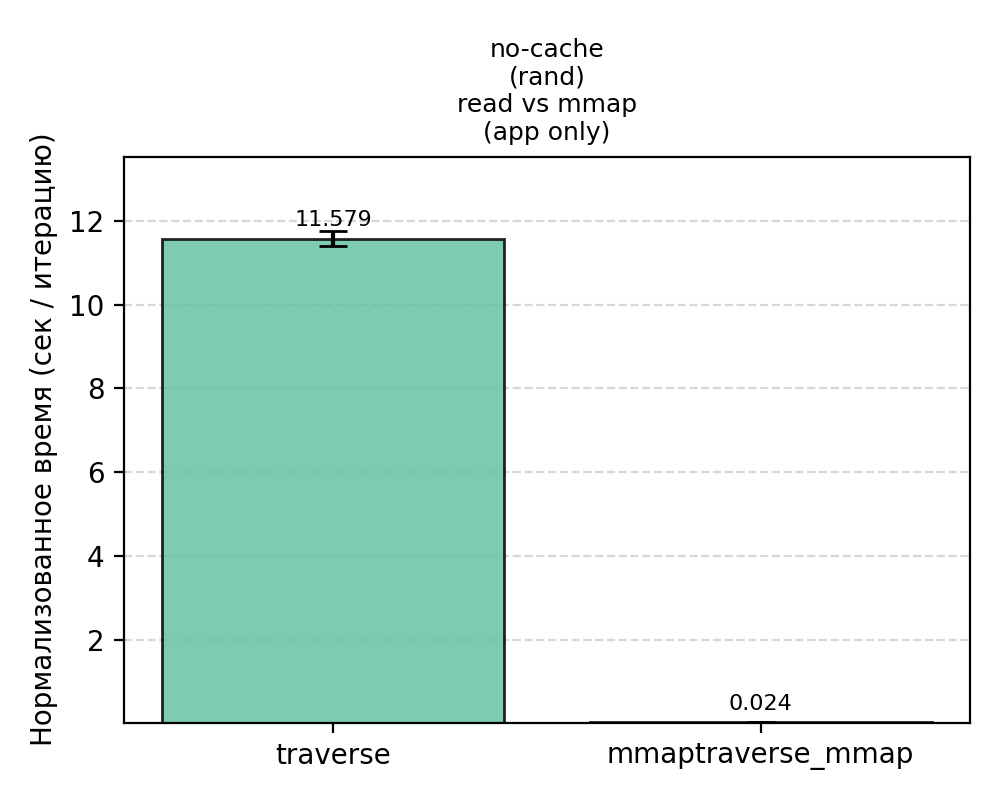
\includegraphics[width=\linewidth]{../graphics/pairwise_8.png}
        \caption{Попарное сравнение 8: read (no-cache) rand vs mmap (no-cache) rand (изменяется только приложение)}
        \label{fig:pair8}
    \end{minipage}
\end{figure}

\begin{figure}[h]
    \centering
    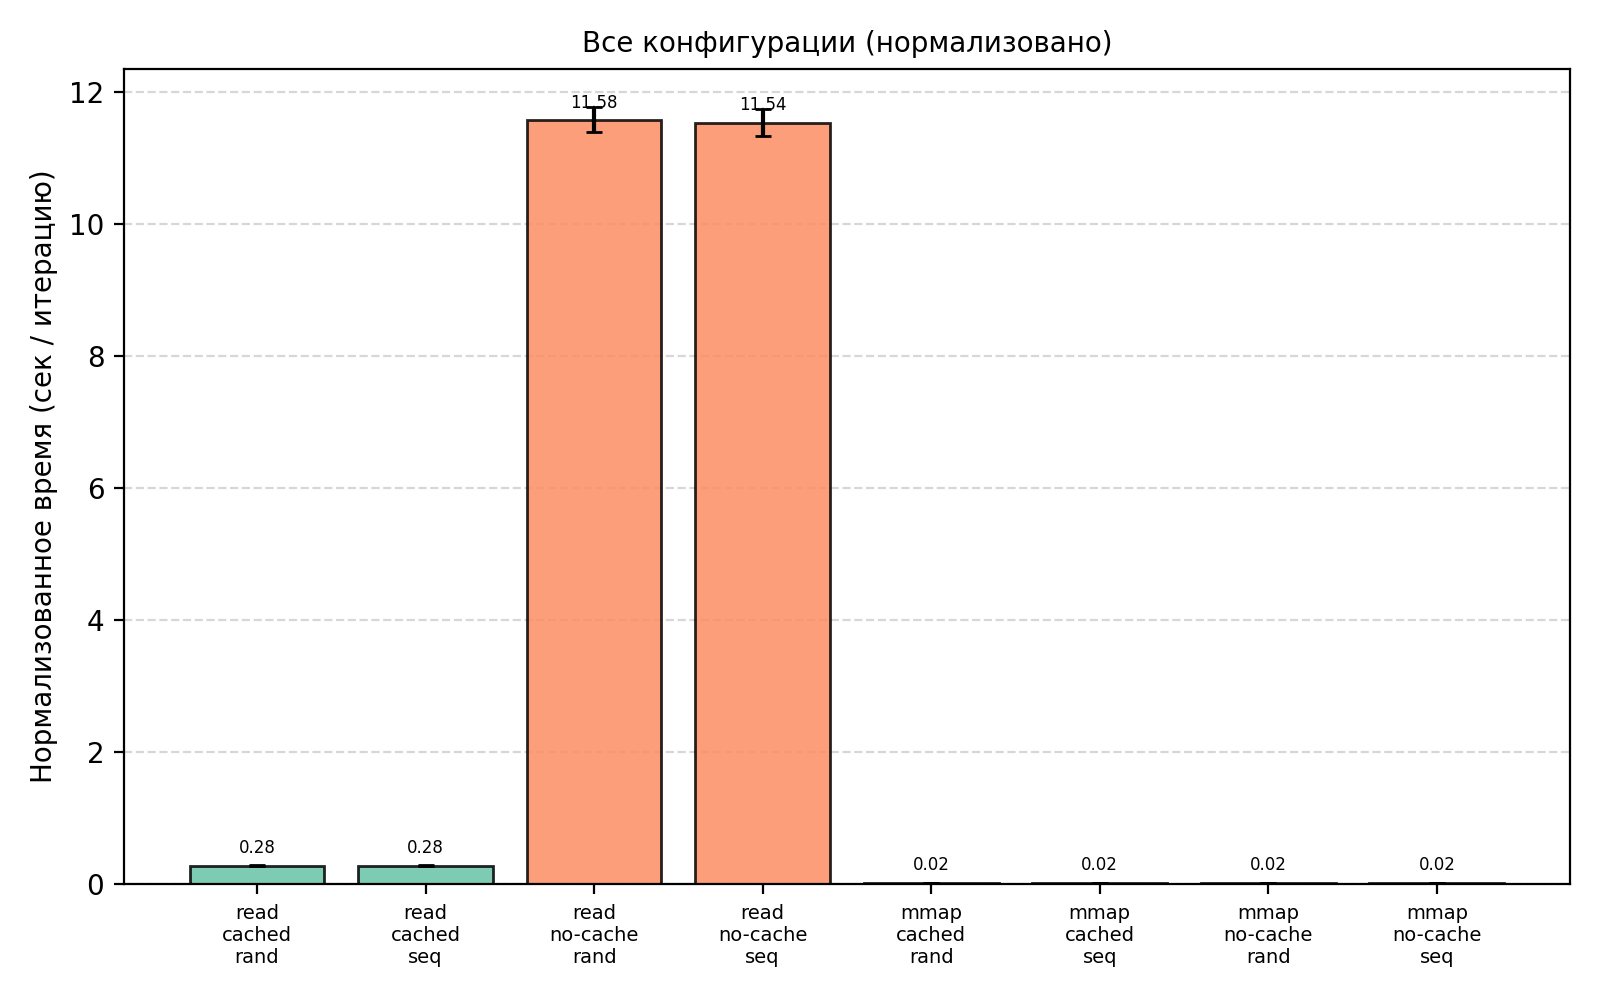
\includegraphics[width=0.9\textwidth]{../graphics/all_config_normalized.png}
    \caption{Все конфигурации (нормализованное время, сек / итерацию)}
    \label{fig:all_config}
\end{figure}

\end{document}